% Appendix Template

\chapter{Project Planning and Budget} % Main appendix title

\label{AppendixC} % Change X to a consecutive letter; for referencing this appendix elsewhere, use \ref{AppendixX}


\lhead{Appendix C. \emph{Project Planning and Budget}} % Change X to a consecutive letter; this is for the header on each page - perhaps a shortened title

\section{Project Planning}

The idea of working on this Thesis started in June of 2013, when Victor, my supervisor, told me the possibility of working in a novelty detection system. During the summer of 2013 I was able to do some research on what novelty detection was and the algorithms used for this purpose. I worked through the ScikitLearn \cite{scikit-learn} tutorials to understand better how they worked.

The main issue in this Thesis, and what took more time, was understanding the problem we were dealing with. It may seem simple at first sight, but to unravel the process of curiosity is not a simple task. From September to December of 2013 I did a lot of tests in the data with different approaches and algorithms that led to nothing during weeks. In October, Victor helped me represent the skeleton data in 3D, and this was a big step in understanding what was really happening in the tests. After more weeks of testing, we discovered that the differences the reference frame for the skeletons was providing erroneous outcomes in the tests. We also discovered that the bad recoding of the legs was an problem, and implemented the preprocessing module.

It was not until February when the complete system was designed, including the steps of noise filtering and strangeness detection. Then, we realized the importance of an adjustable sensitivity in the system, and added the concept of $curiosity$ $factor$. From March until May, the system was tested with different groups of data from the poses dataset.

The planning is divided in the following parts: research of the problem literature and State of the Art; planning; design of the novelty detection system; representation of the dataset in 3D; software design; experiments; memory and presentation. They can be seen in Figure \ref{Gantt}.

Initially, the representation of the dataset in 3D was not in the project planning. However, the design of the novelty detection system was blindfolded without it, since we knew that the system detected novelties but we did not know why of what they represented really. It was necessary to create a branch in the plannification to work on it, and it helped a lot to finish the design of the novelty detection system and then it was key for the experiments.    

The approximate time dedicated to this Thesis was 966 hours. The hours are calculated from June of 2013. 

\begin{itemize}
\item June - September (60 working days - 30 vacation) average of 2 hours working on the project
\item September - November (90 days) average of 3 hours daily
\item December - February (90 days) average of 2 hours daily
\item March - 22 May (82 days) average of 3 hours daily
\item 22 May - 22 June (30 days) average of 5 hours daily
\end{itemize}

There were meetings appointed with my supervisor every week on Thursdays.

\begin{landscape}

The general Project Planning is depicted in Figure \ref{Gantt}. 
\begin{figure}[h]
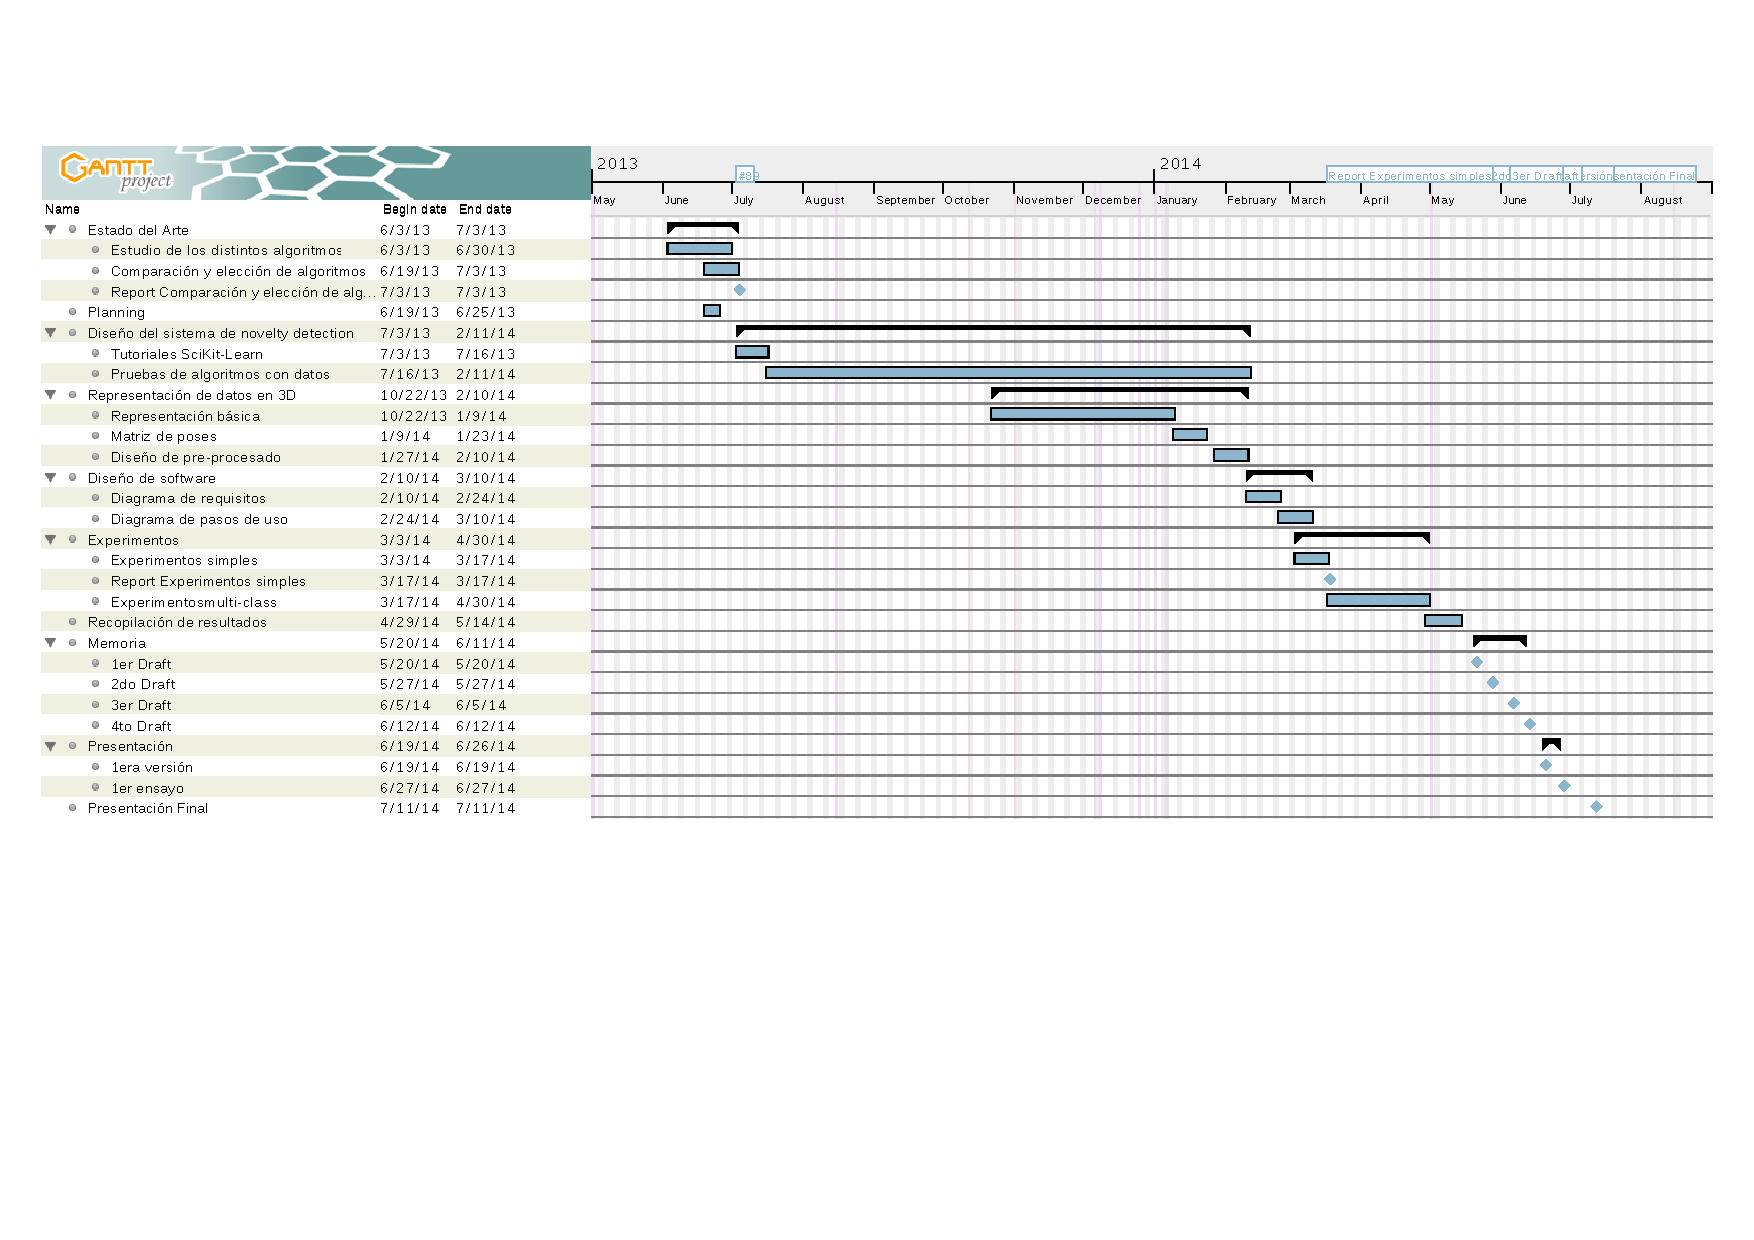
\includegraphics[width=24cm]{Figures/Gantt}
\centering
\caption{Gantt Plan of the Thesis \label{Gantt}}
\end{figure}
\end{landscape}

\section{Project Budget}

The following budget is based on base salaries for a Junior Engineer in Spain, pre taxes, and the hours worked in this Thesis. It was assumed that the working hours in a month are 240, 8 hours per day.

\begin{table}[h]

\centering

\begin{tabular}{lrrrr}
    \toprule
    Description      & Units  & Amount & Unitary price & Total\\
    \midrule
    Junior Engineer   &     h     &   966 & 8 $\geneurowide$   & 7,728 $\geneurowide$ \\
    MacBook Air 13''   &     uds.     &   1 & 1,029 $\geneurowide$   & 1,029 $\geneurowide$ \\
	\\
    \textsc{Total Projected Cost } & & & &\fbox{8,757 $\geneurowide$}\\
    \bottomrule                
\end{tabular}
\caption{Project Budget Estimation}
\end{table}